\problemname{Automatic Accountant}

The bank you work in has purchased an advanced technological solution to the
problems it has with counting money deposited by clients.
The machine works by running each individual coin along a sloped track.
At every integer multiple of centimetres along, starting from $1$cm, there is
a slot in the track with a bucket underneath.

\begin{figure}[h!]
  \centering
  \includegraphics[width=0.4\textwidth]{illustration}
  \label{fig:automaticaccountant}
\end{figure}

The slot will allow a coin to fall in, if
   the thickness of the coin (in millimetres) is
        \textbf{less than or equal to} the width of the slot
        (also in millimetres),
and
   the mass of the coin (in grams) is \textbf{greater than or equal to}
        the trigger mass of the slot (also in grams).

Since the slots are spaced $1cm$ apart centre-to-centre, and since there can be
a large number of coins (or other metal shapes) inserted, the amount of wear
on the track will depend on total distance travelled by all coins.

Given a list of the coins that will be deposited, what total distance will they
travel, in centimetres?

\section*{Input}

The input consists of:
\begin{itemize}
  \item one line containing the number of slots, $s$ ($1 \leq s \leq 10^5 $).
  \item $s$ further lines, the $i$th line containing the width of a slot in millimetres
        and trigger mass in grams of the $i$th slot, $a_i$ and $b_i$ respectively 
        ($1 \le a, b \le 10^5$).
  \item one line containing the integer $c$ ($1 \leq c \leq 10^5 $), the number
        of coins.
  \item $c$ further lines, the $j$th line containing the thickness in millimetres and mass
        in grams of the $j$th coin, $u_i$ and $v_i$ respectively
        ($1 \le u, v \le 10^5$).
\end{itemize}

It is guaranteed that every coin will be able to fall into at least one slot.

\section*{Output}

Output the total distance in centimetres travelled by coins.

